\chapter{Benutzerdokumentation}
\label{ch:4}
\section{Hauptprogramm}
Nach dem Starten des Programms erscheint folgende GUI:

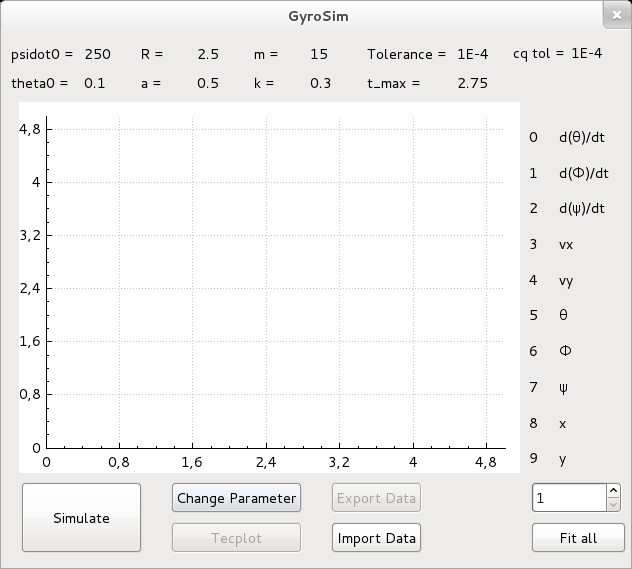
\includegraphics[width=4in,keepaspectratio=true]{figures/mainwindow_clean.png}
\newpage

Mit einem Mouseclick auf 'Change Parameter' \"offnet sich das Parameterfenster:

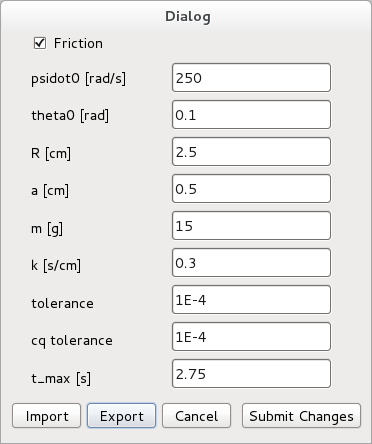
\includegraphics[width=4in,keepaspectratio=true]{figures/change_parameter_default.png}
\newpage

Hier hat der Nutzer die M\"oglichkeit, die Reibung durch Klicken einer Checkbox ein- bzw. auszuschalten.

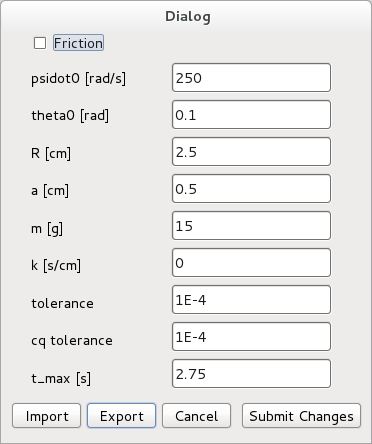
\includegraphics[width=4in,keepaspectratio=true]{figures/parameterwindow_nofriction.png}
\newpage

Ebenso kann er eine Parameterkonfiguration als $*.par$ exportieren und wieder importieren.

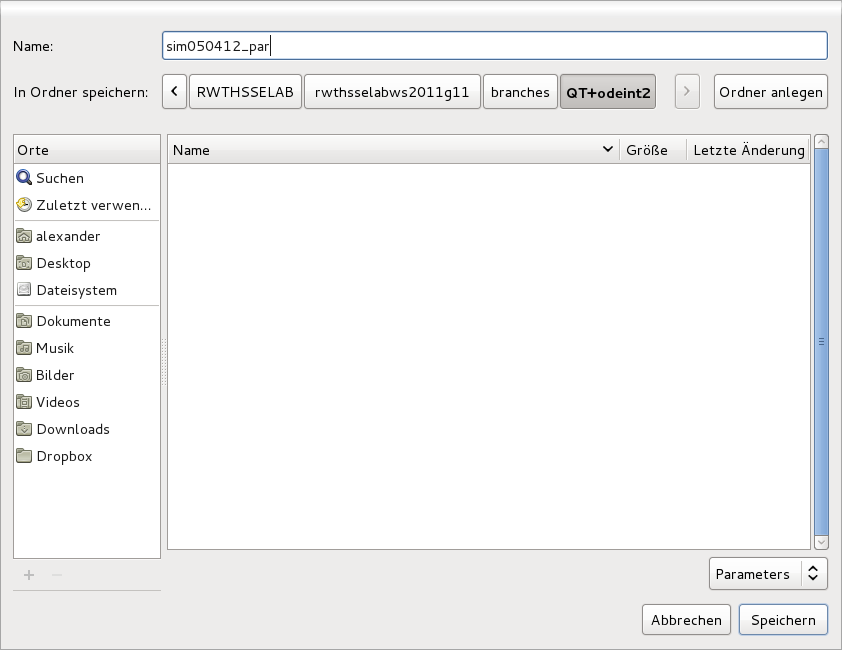
\includegraphics[width=4in,keepaspectratio=true]{figures/export_par.png} 
\newpage

Nachdem die Parameter mit dem Button 'Submit Changes' gesetzt worden sind, klickt der Nutzer im Hauptfenster auf 'Simulate' und nachdem die Berechnung durch das Programm erfolgt ist, erscheint der erste Graph $\dot \theta$.

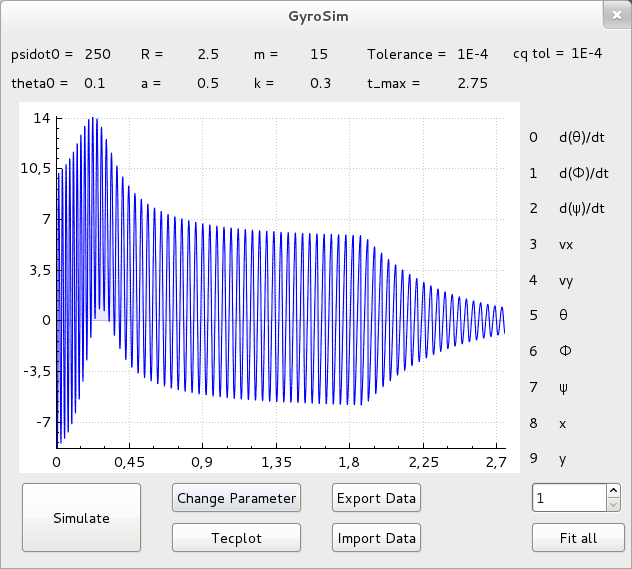
\includegraphics[width=4in,keepaspectratio=true]{figures/mainwindow_after_sim_klicked.png}
\newpage

Der Nutzer kann sich auch alle anderen Graphen anzeigen lassen:

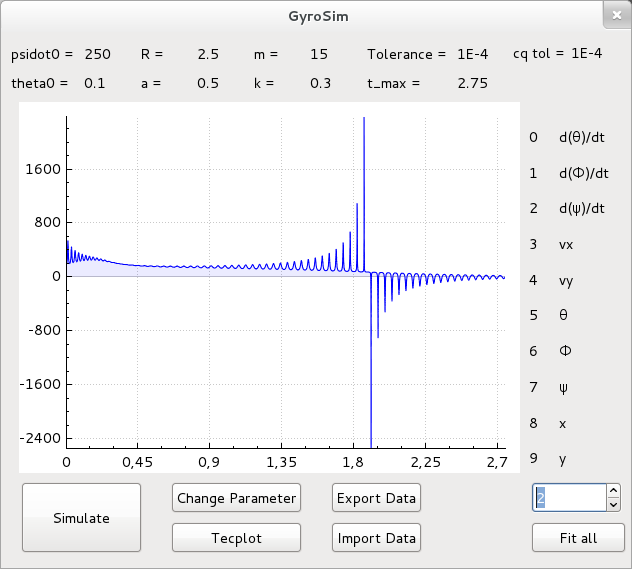
\includegraphics[width=2in,keepaspectratio=true]{figures/mainwindow_g2.png}

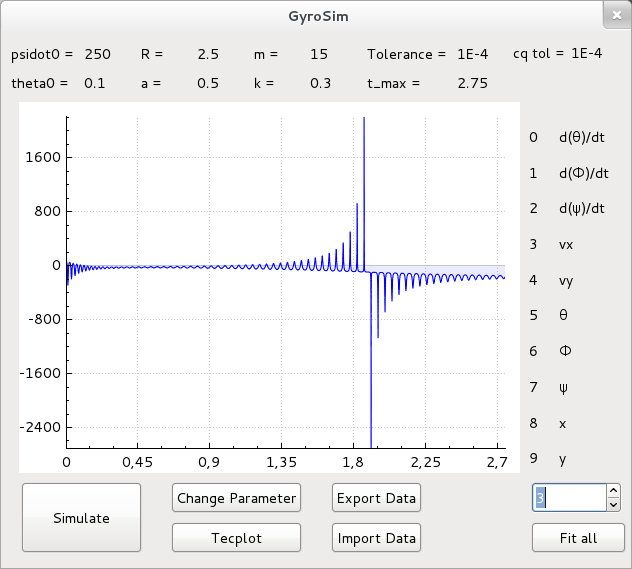
\includegraphics[width=2in,keepaspectratio=true]{figures/mainwindow_g3.png}

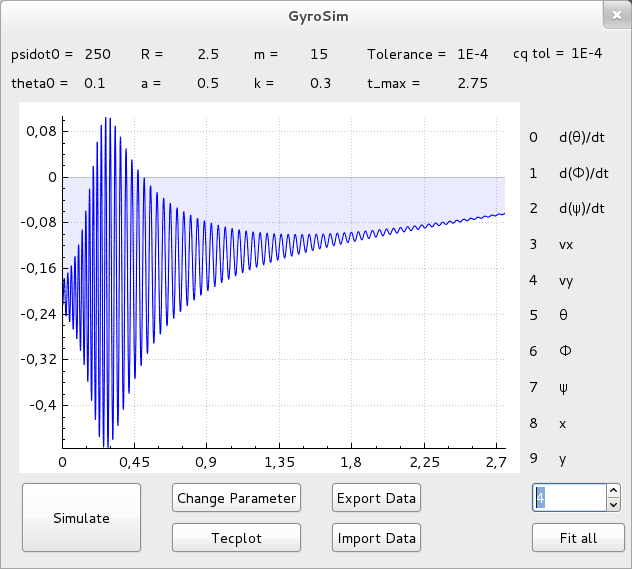
\includegraphics[width=2in,keepaspectratio=true]{figures/mainwindow_g4.png}

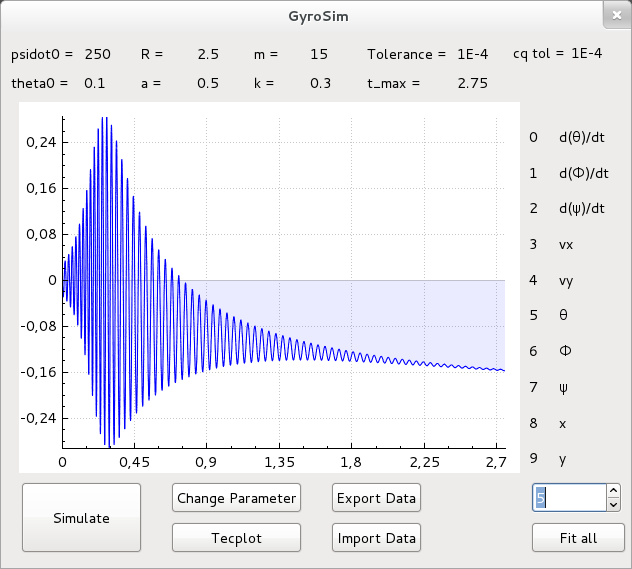
\includegraphics[width=2in,keepaspectratio=true]{figures/mainwindow_g5.png}

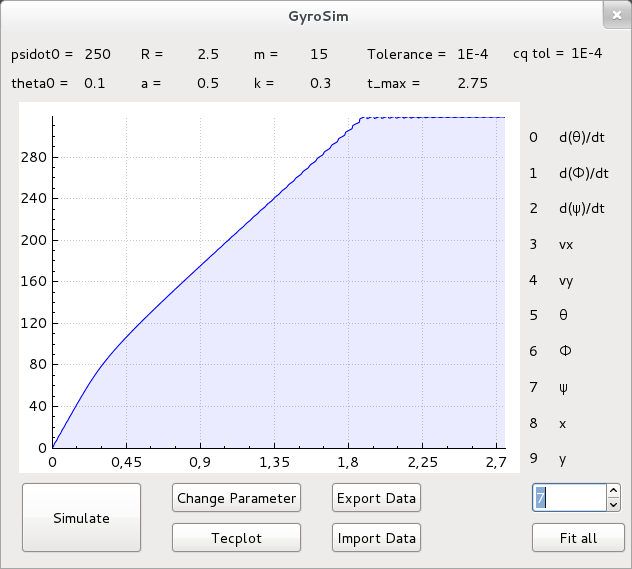
\includegraphics[width=2in,keepaspectratio=true]{figures/mainwindow_g7.png}

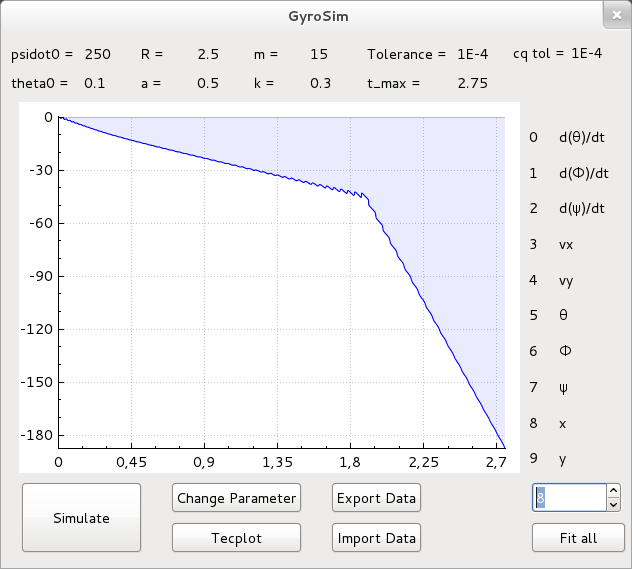
\includegraphics[width=2in,keepaspectratio=true]{figures/mainwindow_g8.png}

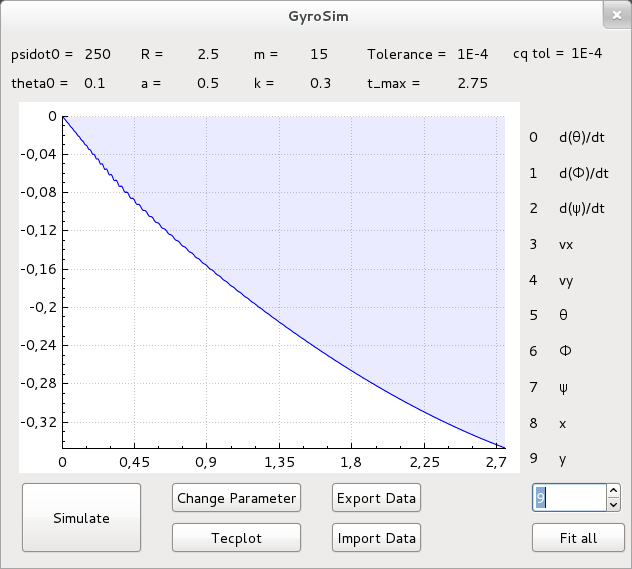
\includegraphics[width=2in,keepaspectratio=true]{figures/mainwindow_g9.png}

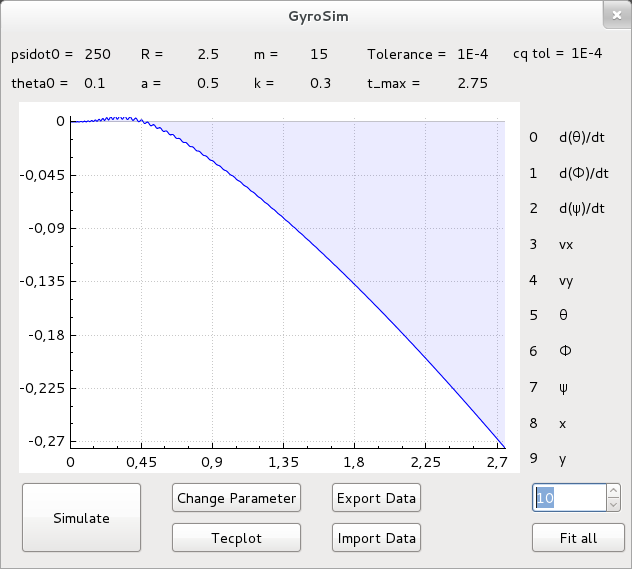
\includegraphics[width=2in,keepaspectratio=true]{figures/mainwindow_g10.png}
\newpage

Im Hauptfenster kann der Nutzer nach erfolgter Simulation die Daten entweder als Tecplot oder als $*.gyro$ speichern und bereits exportierte Daten wieder importieren.

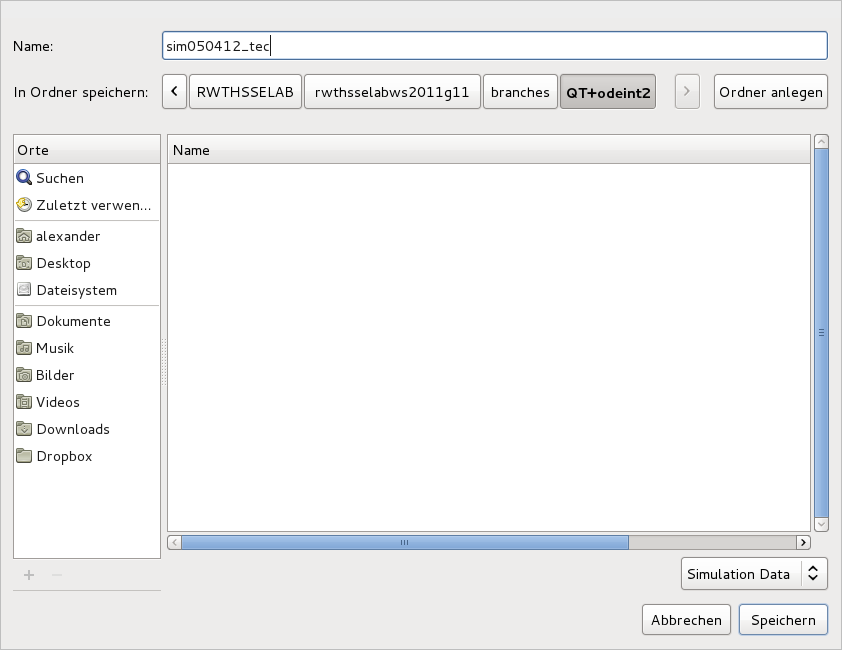
\includegraphics[width=2in,keepaspectratio=true]{figures/exportdialog_tec.png}

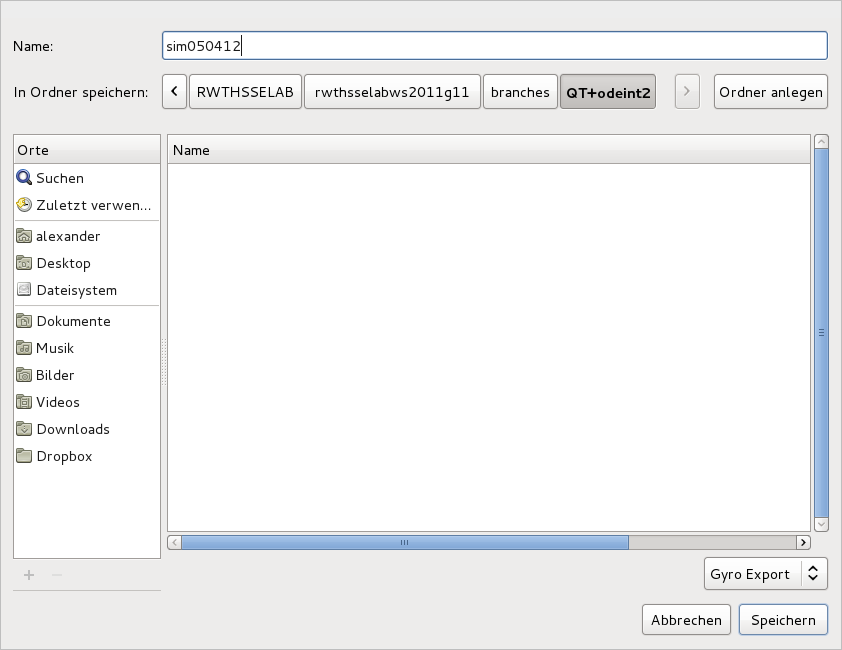
\includegraphics[width=2in,keepaspectratio=true]{figures/export_data.png}

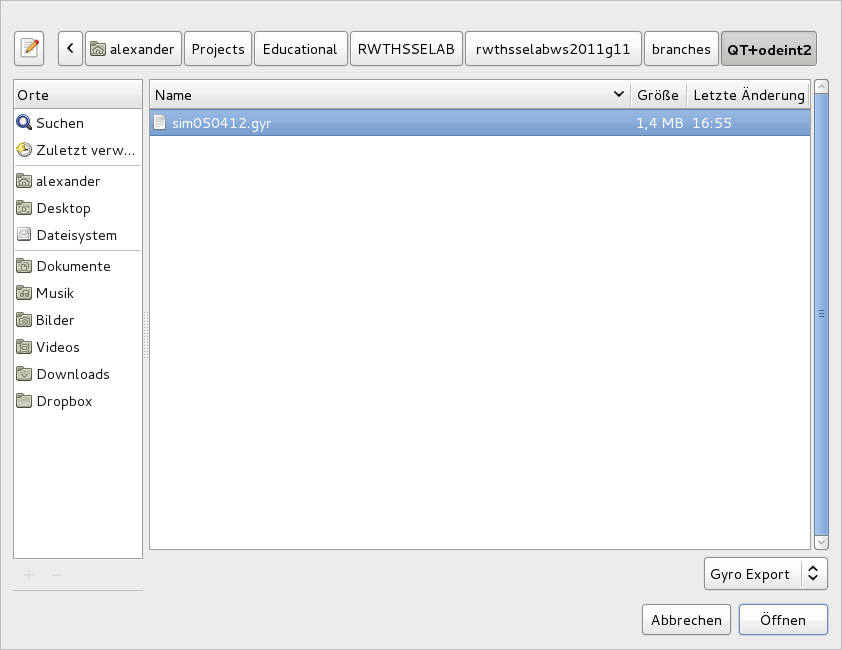
\includegraphics[width=2in,keepaspectratio=true]{figures/import_data.png}
\newpage

\section{Fehlermeldungen}
Bei physikalisch falschen Eingaben erfolgt eine Fehlermeldung.

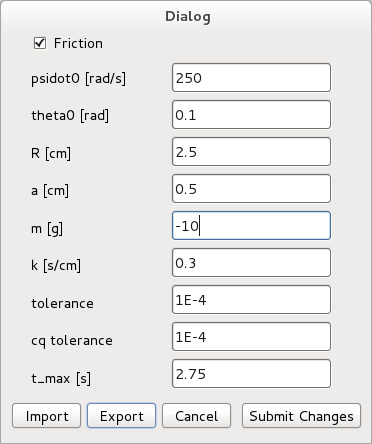
\includegraphics[width=2in,keepaspectratio=true]{figures/change_parameter_negative_mass.png}

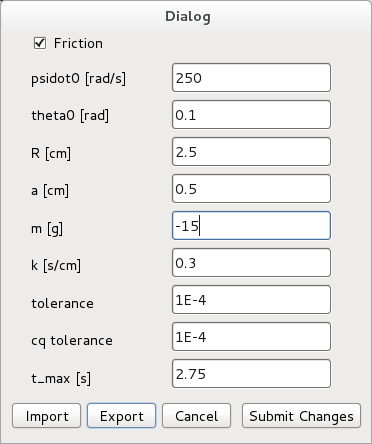
\includegraphics[width=2in,keepaspectratio=true]
{figures/paremeter_window_negative_mass.png}

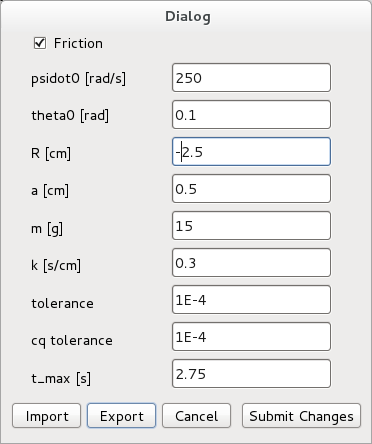
\includegraphics[width=2in,keepaspectratio=true]{figures/paremeter_window_negative_R.png}

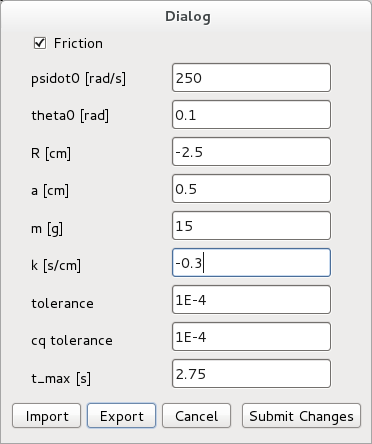
\includegraphics[width=2in,keepaspectratio=true]{figures/paremeterwindow_negative_k.png}
\medskip

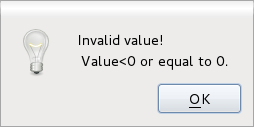
\includegraphics[width=3in,keepaspectratio=true]{figures/parameter_window_parameter_exception.png}

